\begin{tikzpicture}[scale=0.8, transform shape]
	\onslide<1->{ % node[below=2]
		
		\draw[draw=blue!50,fill=cyan!10,thick,solid,rounded corners] (3.3,4.6) rectangle (0.7,7.3);    

		\node[inner sep=0pt] (A) at (2,6)
		{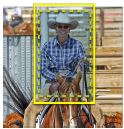
\includegraphics[scale=0.7]{images/CNN_cowboy.JPG}};}

	\onslide<2->{
		\draw[draw=blue!50,fill=cyan!10,thick,solid,rounded corners] (5.3,4.8) rectangle (3.7,7.2);    

		\node[inner sep=0pt] (B) at (4.5,6)
		{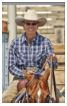
\includegraphics[scale=0.7]{images/CNN_cowboy_crop.JPG}};
		\node at (4.5,4.5) {};}
	\onslide<2->{\draw[black, thick, ->]  (3.2,6) --  (3.9,6);} 
	
	
	\onslide<3->{
		\draw[draw=blue!50,fill=cyan!10,thick,solid,rounded corners] (8.3,4.8) rectangle (5.9,7.2);    

		\node[inner sep=0pt] (C) at (7.1,6)
		{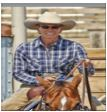
\includegraphics[scale=0.7]{images/CNN_cowboy_scale.JPG}};
		\node [text width=35mm] at (7.8,4) {};
	}
	\onslide<3->{\draw[black, thick, ->]  (5.2,6) --  (6.1,6);} 
	
\end{tikzpicture}
